%Papers for top-Higgs Yukawa coupling, tth, and the analysis process: 
%https://arxiv.org/pdf/1807.02441.pdf
%http://cds.cern.ch/record/1690648/files/LCD_tth_note.pdf?version=1
%http://cds.cern.ch/record/1982243/files/CLICdp-Note-2015-001.pdf?version=1
%https://arxiv.org/pdf/1608.07538.pdf

\chapter{Physics studies for the Compact Linear Collider}
\label{chapter:analysis}

\epigraph{Somewhere, something incredible is waiting to be known.}{Carl Sagan}

This chapter will discuss the usage of full-scale detector simulations to assess the performance of the proposed \acrshort{CLIC}\textunderscore \acrshort{SiD} detector at the \acrlong{CLIC} machine, during the later stages where centre of mass energies in the tera-scale are possible.

This work was done with the \acrfull{CLICdp} collaboration to determine the uncertainty on the measurement of the top-Higgs Yukawa coupling in the $e^+ e^- \rightarrow t\overline{t}H$ process at a centre of mass energy of $\sqrt{s}$ = 1.4 TeV, using the \acrshort{CLIC}\textunderscore \acrshort{SiD} detector concept. The analysis as discussed here focuses specifically on the hadronic decay channel, where both top quarks decay to a W boson and bottom quark, and both W bosons decay hadronically. When taken in combination with a similar analysis of the semi-leptonic channel performed by Yixuan Zhang, this allows the expected uncertainty on the top-Higgs Yukawa coupling to be calculated.

This analysis was an update of an earlier study into the sensitivity of the \acrshort{SiD} to the top-Higgs Yukawa coupling \cite{clic-yukawa-coupling-2014}. The analysis presented here used an updated version of the flavour-tagging software, and a better determination of the contributions of the higgstrahlung diagram.

These results were then contributed to a paper that summarised the top physics potential for \acrshort{CLIC} at $\sqrt{s}$ = 1.4 TeV, which was submitted to \acrshort{CERN}'s European Strategy Update in 2019 \cite{clic-top-quark-physics} \cite{clic-2018-summary}.

\section{Introduction}
One of the primary goals of all the future lepton colliders discussed in Chapter \ref{chapter:colliders} is to become ``Higgs factories'' -- machines that can produce large numbers of Higgs bosons in a variety of final states, allowing the Higgs sector of the \acrlong{SM} to be probed with unprecedented accuracy and coverage.

One of the best ways to examine the Higgs sector is via the production of Higgs bosons in association with top quarks. The coupling between these two particles is the strongest Higgs coupling in the \acrshort{SM}, making it one of the easiest ways to examine the properties of the Higgs boson and the Higgs sector. This is the top-Higgs Yukawa coupling $y_t$. The \acrlong{SM} predicts the value of the top-Higgs Yukawa coupling to be:

\begin{equation}
	y_t^{SM} = \frac{\sqrt{2m_t}}{v}
\label{eq:yukawacoupling-sm-value}
\end{equation}

where $m_t$ is the mass of the top quark and $v$ is the vacuum expectation value of the Higgs potential. Many models for new physics predict a deviation from the \acrshort{SM} value, e.g two Higgs-doublet models, the \acrfull{MSSM}, as well as composite Higgs or Little Higgs models \refthis . Determining the top-Higgs Yukawa coupling will provide an important test of both the \acrlong{SM} and a multitude of these new physics models. The various detector models for future lepton colliders will enable this coupling to be measures at the percent level, making this a strong physics motivation for these machines.

The process used for studying the top-Higgs Yukawa coupling is the $e^+ e^- \rightarrow t\overline{t}H$ process, also referred to as the tth process. This allows measurement of the coupling due to the direct interaction between the top quark and Higgs boson at the vertex.

In order to calculate the uncertainty on the coupling, the uncertainty of the cross-section of the tth process must first be calculated, and this can then be converted into the coupling:

\begin{equation}
	\frac{\Delta y_t}{y_t} = \kappa \frac{\Delta \sigma}{\sigma}
\label{eq:crosssection-to-yukawa}
\end{equation}

where $\sigma$ is the cross-section of the process, and $\kappa$ is some prefactor, normally assumed to be 0.5. This means that by determining the uncertainty on the cross-section of the tth process $\frac{\Delta \sigma}{\sigma}$, the uncertainty on the coupling can be determined directly in a model-independent manner. 

% This says that k is a factor but what is its origin? Please clarify that this kappa factor is theoretical in its origin. Also, clarify the kappa factor from the previous version of this analysis and how much of the 11% improvement that you find in your study comes from the change in kappa factor from (you said) 0.53 to 0.503.

\section{The $e^+ e^- \rightarrow t\overline{t}H$ process}
The tth process offers one of the best ways to examine the interaction of the Higgs boson and the top quark, due to the direct interaction between the two at the vertex where the Higgs boson is radiated from the top quark. This process is also uniquely accessible to the linear lepton colliders, as the production threshold is on the order of ~500 GeV, above the maximum design energy of both the \acrshort{FCC}-ee and the \acrshort{CEPC}.

\begin{figure}[h]
	\centering
	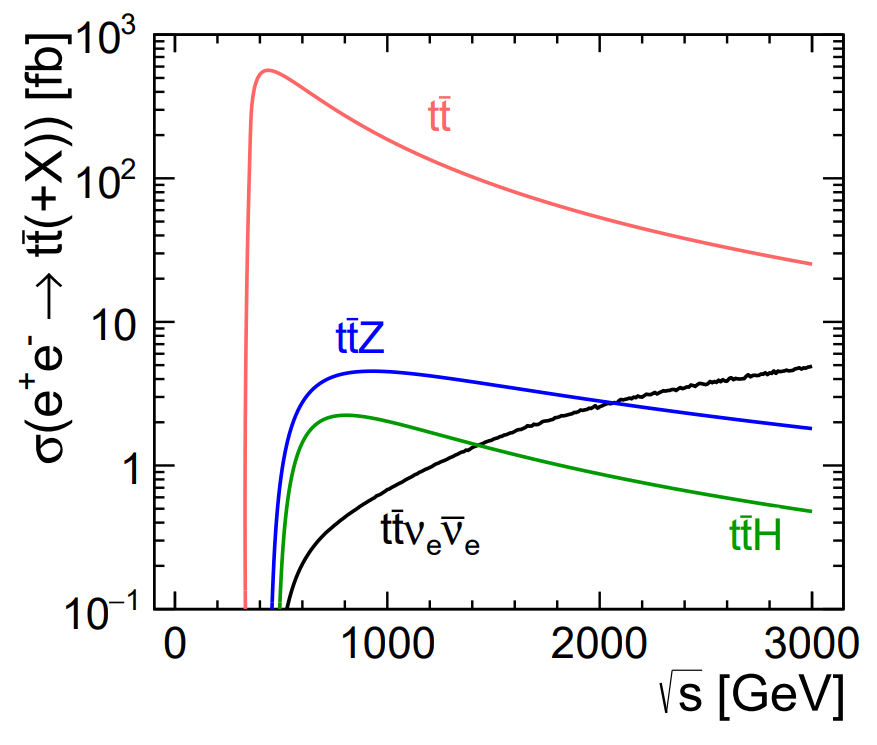
\includegraphics[width=0.55\textwidth]{../Pictures/Analysis/tt-production-crosssection.png}
	\caption{The cross-section of various top-quark pair production processes at a lepton collider. This plot assumes a top quark mass of $m_t$ = 174 GeV and a Higgs boson mass of $m_H$ = 125 GeV, as well as unpolarised beams. The $t\overline{t}$ and $t\overline{t}Z$ processes are important backgrounds for this analysis. \refthis}
	\label{figure:analysis/top-quark-plot}
\end{figure}

The final states of the tth process are complicated due to the variety of decay modes of the particles. In the analysis considered here, the two top quarks are permitted to decay only via the $t \rightarrow W^+ b $ process. The bottom quark forms a jet, while the W boson has all possible decay processes. W bosons can decay \textit{hadronically} into a pair of one up-type quark and one down-type quark (e.g. $u\overline{d}$ or $c\overline{s}$). Or they can decay \textit{leptonically} into a charged lepton and a neutrino of the same flavour (e.g. $e^- \overline{\nu}_e$ or $\mu^+ \nu_\mu$). The total branching ratio of all hadronic decays is 68\%, and the total branching ratio of all leptonic decays is 32\% \cite{pdg-review}. We denote a quark-antiquark pair as $q\overline{q}$, and a lepton-neutrino pair as $\ell \nu$.

Given that we focus only on events where the Higgs decays via the process $H \rightarrow b\overline{b}$, there are then three possible final states: %Redid these, double check once rendered
$$e^+ e^- \rightarrow t\overline{t}H \rightarrow q\overline{q}q\overline{q}b\overline{b}$$
$$e^+ e^- \rightarrow t\overline{t}H \rightarrow \ell \nu q \overline{q} b \overline{b}$$
$$e^+ e^- \rightarrow t\overline{t}H \rightarrow \ell \nu \ell \nu b \overline{b}$$

Due to the branching ratios, the hadronic and semi-leptonic final states are the most common, and the leptonic final state occurs less than ten percent of the time. This means that the most common final states all heavily rely upon jets, meaning that in order to perform accurate analysis of this process, jet energy resolution and jet reconstruction is of primary importance. As discussed in Chapter \ref{chapter:colliders}, the detector concepts for future lepton colliders are designed to focus on jet energy resolution and jet reconstruction, and utilise particle flow to augment this. \\

\begin{figure}[h]
	\centering
	\begin{tikzpicture}[line width=1.3 pt,scale=2]
		\draw[fermion]  (0,1) -- (1,0) ;
		\draw[fermionbar]  (0,-1) -- (1,0) ;
		\draw[vector]  (1,0) -- (2.5,0) ;
		\draw[fermion]  (2.5,0) -- (3.5,1) ;
		\draw[fermionbar]  (2.5,0) -- (3.5,-1) ;
		\draw[scalar]  (2.75,0.25) -- (3.5,0.) ;
		\node at (-0.3, 1) {$e^-$};
		\node at (-0.3, -1) {$e^+$};
		\node at (3.8, 1) {$t$};
		\node at (3.8, -1) {$\overline{t}$};
		\node at (3.8, 0) {$H$};
		\node at (1.75, 0.3) {$Z/\gamma *$};
	\end{tikzpicture} 
	\caption{Feynman diagram of the tth event.}
	\label{figure:physics/SM/feynman-tth}
\end{figure}

There are significant irreducible backgrounds in the form of the $t\overline{t}Z$ and $t\overline{t}b\overline{b}$ processes, both of which are able to produce similar decays with 2, 4 or 6 leptons in the final state. These processes form a large contribution to the background due to their large cross-sections. The $t\overline{t}$ process is also a huge contribution to background because of its extremely high cross-section. 

\subsection{Higgstrahlung}
\label{section:higgstrahlung}
There is also another contribution to the tth final state in the form of \textit{higgstrahlung}. This process is actually an $e^+e^- \rightarrow t\overline{t}$ event where the intermediate $Z/\gamma *$ radiates a Higgs boson \textit{before} producing the $t\overline{t}$ pair (see Fig. \ref{figure:physics/SM/higgstrahlung}). This means the final state is tth but there is no vertex between the top quark and Higgs, meaning this process is not sensitive to the coupling. 

If these events are not accounted for when calculating the cross-section of the tth process, the precision of the coupling measurement will be overestimated, as it is counting the higgstrahlung events that are not sensitive to the coupling and do not contribute to it.

The effects of higgstrahlung are accounted for by the value of the prefactor $\kappa$ from Equation \ref{eq:crosssection-to-yukawa}. If the contribution from higgstrahlung is negligible, then $\kappa$ = 0.5. When the effect is significant, the value of $\kappa$ will become greater than 0.5. 

% Get better "approx less than or equal to" sign
This contribution is energy-dependent and at lower energies ($\sqrt{s}$ $\leqslant$ $\sim 500$ GeV) it is assumed to be negligible. However, for energies above 1 TeV, higgstrahlung contributes a non-negligible number of tth events and must be accounted for.

% Need to introduce or discuss or use references for terms such as NLO to NNLO? beamstrahlung also not introduced so far either?
For this analysis, new work using NLO corrections to \acrshort{QCD}, initial state radiation, and beamstrahlung effects, determined that $\kappa$ = 0.503 \cite{kappa-NLOQCD}. \\

\begin{figure}[h]
	\centering
	\begin{tikzpicture}[line width=1.3 pt,scale=2]
		\draw[fermion]  (0,1) -- (1,0) ;
		\draw[fermionbar]  (0,-1) -- (1,0) ;
		\draw[vector]  (1,0) -- (2.5,0) ;
		\draw[fermion]  (2.5,0) -- (3.5,1) ;
		\draw[fermionbar]  (2.5,0) -- (3.5,-1) ;
		\draw[scalar]  (1.75,0) -- (2.5,-1.) ;
		\node at (-0.3, 1) {$e^-$};
		\node at (-0.3, -1) {$e^+$};
		\node at (3.8, 1) {$t$};
		\node at (3.8, -1) {$\overline{t}$};
		\node at (2.8, -1) {$H$};
		\node at (1.75, 0.3) {$Z/\gamma *$};
	\end{tikzpicture} 
	\caption{Feynman diagram of the higgstrahlung process.}
	\label{figure:physics/SM/higgstrahlung}
\end{figure}

\section{Generation of Monte Carlo samples}
The samples used for the study had been generated using ILCDIRAC\cite{ilc-dirac}. The physics generation was done predominantly in WHIZARD 1.95\cite{whizard}, using PYTHIA 6.422\cite{pythia} for the simulation of hadronisation and fragmentation. Due to constraints of WHIZARD, samples with final states with eight fermions were generated in \textsc{PhysSim} \cite{physsim} , also using PYTHIA. The mass of the Higgs boson was set at 125.0 GeV, and the mass of the top quark at 174.0 GeV. 

All samples were simulated at $\sqrt{s}$ = 1.4 TeV using unpolarised beams, assuming an integrated luminosity of 1.5 ab\textsuperscript{-1}. See Table \ref{table:physics/SM/generatedsamples} for a summary of all of the samples used. 

Following the generation of the underlying physics events, the interactions of the particles with the detector must be simulated. This was done using the \textsc{Geant4} toolkit\cite{geant4}, specifically using the \textsc{Mokka} tool. Simulation of the signals that result from the interactions in the detector was done in \textsc{Marlin}\cite{marlin}.

At the end of this process, the Monte Carlo dataset is in a format identical to how information from the constructed detector would look. At this stage, the analysis can proceed as if the data were real. However, in addition to the simulated detector response, there is also the Monte Carlo truth information, which allows correlation of the simulated detector response data with the ``true'' particles in the simulation itself. However, this is not used in this analysis.
% Here or when discussing lepton ID, clarify where truth information is used.

The samples were then given weights associated with their expected cross-sections in femtobarns (fb), assuming an integrated luminosity of 1.5 ab\textsuperscript{-1}. See Table \ref{table:physics/SM/generatedsamples} for a summary of all the generated samples, their cross-sections, sample weights, and expected number of events. \\

% Clarify whether these are 6-fermion samples or process/diagram generations that neglect interference between the different states.  Check CLICdp twiki pages (or ask me) for details.
\begin{table}[htp]
\centering
	\begin{tabular}{ c l c r r }
	\hline \hline
	\textbf{ProdID} & \textbf{Process} & \textbf{Cross-section (fb)} & \textbf{Sample weight} & \textbf{Events in 1.5 ab\textsuperscript{-1}} \\ \hline
	2435 & $t\overline{t}h$, 6 jets, $h \rightarrow b\overline{b}$ & 0.431 & 0.03 & 647 \\
	2441 & $t\overline{t}h$, 4 jets, $h \rightarrow b\overline{b}$ & 0.415 & 0.03 & 623 \\ \hline
	2429 & $t\overline{t}h$, 2 jets, $h \rightarrow b\overline{b}$ & 0.100 & 0.006 & 150 \\

	2438 & $t\overline{t}h$, 6 jets, $h \not\rightarrow b\overline{b}$ & 0.315 & 0.02 & 473	 \\
	2444 & $t\overline{t}h$, 4 jets, $h \not\rightarrow b\overline{b}$ & 0.303 & 0.02 & 455 \\
	2432 & $t\overline{t}h$, 2 jets, $h \not\rightarrow b\overline{b}$ & 0.073 & 0.004 & 110 \\

	2450 & $t\overline{t}Z$, 6 jets & 1.895 & 0.1 & 2843 \\
	2453 & $t\overline{t}Z$, 4 jets & 1.825 & 0.1 & 2738 \\
	2447 & $t\overline{t}Z$, 2 jets & 0.439 & 0.03 & 659 \\
	
	2423 & $t\overline{t}b\overline{b}$, 6 jets & 0.549 & 0.03 & 824 \\
	2426 & $t\overline{t}b\overline{b}$, 4 jets & 0.529 & 0.03 & 794 \\
	2420 & $t\overline{t}b\overline{b}$, 2 jets & 0.127 & 0.008 & 191 \\

	2417 & $t\overline{t}$ & 125.8 & 1.5 & 203700 \\ \hline \hline

	\end{tabular}
	\caption{Table of all signal and background samples used for this analysis. The first two rows are the signal samples, the others are backgrounds.}
	\label{table:physics/SM/generatedsamples}
\end{table}

\section{Event reconstruction}
The tth event has three possible final states, defined by the decay channels of the W bosons produced by the top quarks. The decay of a top quark will always produce a W boson and a bottom quark. Ignoring the decay of the Higgs boson, there are three possible combinations of final states that can be seen in Table \ref{table:physics/final-states}. \\

% This information in table 5.2 would be better presented before table 5.1, where the backgrounds and signals are classified in terms of no. of jets?  Please consider re-ordering the information in the early part of this chapter. Could also include a few more Feynman diagrams to illustrate background processes, some of which are identical final state to signal, and some of which can be reconstructed to appear the same.

\begin{table}[h]
\centering
	\begin{tabular}{ l c c c r }
	\hline \hline
	Decay Channel & Final State & No. of leptons & No. of jets & Branching Ratio \\ \hline
	Fully hadronic & $q\overline{q}q\overline{q}b\overline{b}$ & 0 & 6 & 46\% \\
	Semi-leptonic &  $\ell \nu q\overline{q}b\overline{b}$ & 1 & 4 & 45\% \\
	Fully leptonic & $\ell \nu \ell \nu b\overline{b}$ & 2 & 2 & 9\% \\ \hline \hline
	\end{tabular}
	\caption{ }
	\label{table:physics/final-states}
\end{table}

Given the low branching ratio compared to the other channels, the fully leptonic state is not used in this analysis. Feynman diagrams of the fully hadronic and semi-leptonic final states are shown in Figs. \ref{figure:physics/SM/feynman-tth-hadronic} and \ref{figure:physics/SM/feynman-tth-semileptonic}

\begin{figure}
	\centering
	\begin{tikzpicture}[line width=1.3 pt,scale=2.25]
		% Initial electrons	
		\draw[fermion]  (0,1) -- (1,0) ;
		\draw[fermionbar]  (0,-1) -- (1,0) ;
		% The central bar
		\draw[vector]  (1,0) -- (2.5,0) ;
		% The final top quarks
		\draw[fermion]  (2.5,0) -- (3.5,1) ;
		\draw[fermionbar]  (2.5,0) -- (3.5,-1) ;
		% The Higgs boson radiating off
		\draw[scalar]  (2.75,0.25) -- (3.5,0.) ;
		% The W+ and bottom quark coming off the top quark
		\draw[vector]  (3.5,1) -- (4.5,1.5) ;
		\draw[fermion]  (3.5,1) -- (4.5,0.5) ;
		% The W- and anti-bottom quark coming off the anti-top quark
		\draw[fermionbar]  (3.5,-1) -- (4.5,-0.5) ;
		\draw[vector]  (3.5,-1) -- (4.5,-1.5) ;
		% The quark-antiquark pair coming off the W+
		\draw[fermion]  (4.5, 1.5) -- (5.5,2) ;
		\draw[fermion]  (4.5, 1.5) -- (5.5,1) ;
		% The quark-antiquark pair coming off the W-
		\draw[fermionbar]  (4.5, -1.5) -- (5.5,-1) ;
		\draw[fermionbar]  (4.5, -1.5) -- (5.5,-2) ;
		% Labels
		\node at (-0.3, 1) {$e^-$};
		\node at (-0.3, -1) {$e^+$};
		\node at (3.8, 1) {$t$};
		\node at (3.8, -1) {$\overline{t}$};
		\node at (3.8, 0) {$H^0$};
		\node at (5.0, 1.5) {$W^+$};
		\node at (4.8, 0.5) {$b$};
		\node at (4.8, -0.5) {$\overline{b}$};
		\node at (5.0, -1.5) {$W^-$};
		\node at (5.8,2) {$q$};
		\node at (5.8,1) {$\overline{q}$};
		\node at (5.8,-1) {$q$};
		\node at (5.8,-2) {$\overline{q}$};
	\end{tikzpicture} 
	\caption{Feynman diagram of the tth event, showing the fully-hadronic decay channel with the final state $q\overline{q}q\overline{q}b\overline{b}$. \newline}
	\label{figure:physics/SM/feynman-tth-hadronic}
	\begin{tikzpicture}[line width=1.3 pt,scale=2.25]
		% Initial electrons
		\draw[fermion]  (0,1) -- (1,0) ;
		\draw[fermionbar]  (0,-1) -- (1,0) ;
		% The central bar
		\draw[vector]  (1,0) -- (2.5,0) ;
		% The final top quarks
		\draw[fermion]  (2.5,0) -- (3.5,1) ;
		\draw[fermionbar]  (2.5,0) -- (3.5,-1) ;
		% The Higgs boson radiating off
		\draw[scalar]  (2.75,0.25) -- (3.5,0.) ;
		% The W+ and bottom quark coming off the top quark
		\draw[vector]  (3.5,1) -- (4.5,1.5) ;
		\draw[fermion]  (3.5,1) -- (4.5,0.5) ;
		% The W- and anti-bottom quark coming off the anti-top quark
		\draw[fermionbar]  (3.5,-1) -- (4.5,-0.5) ;
		\draw[vector]  (3.5,-1) -- (4.5,-1.5) ;
		% The lepton-neutrino pair coming off the W+
		\draw[fermion]  (4.5, 1.5) -- (5.5,2) ;
		\draw[fermion]  (4.5, 1.5) -- (5.5,1) ;
		% The quark-antiquark pair coming off the W-
		\draw[fermionbar]  (4.5, -1.5) -- (5.5,-1) ;
		\draw[fermionbar]  (4.5, -1.5) -- (5.5,-2) ;
		% Labels
		\node at (-0.3, 1) {$e^-$};
		\node at (-0.3, -1) {$e^+$};
		\node at (3.8, 1) {$t$};
		\node at (3.8, -1) {$\overline{t}$};
		\node at (3.8, 0) {$H^0$};
		\node at (5.0, 1.5) {$W^+$};
		\node at (4.8, 0.5) {$b$};
		\node at (4.8, -0.5) {$\overline{b}$};
		\node at (5.0, -1.5) {$W^-$};
		\node at (5.8,2) {$\ell$};
		\node at (5.8,1) {$\nu$};
		\node at (5.8,-1) {$q$};
		\node at (5.8,-2) {$\overline{q}$};
	\end{tikzpicture} 
	\caption{Feynman diagram of the tth event, showing the semi-leptonic decay channel  with the final state $\ell\nu q\overline{q}b\overline{b}$.}
	\label{figure:physics/SM/feynman-tth-semileptonic}
\end{figure}

\subsection{Lepton identification}
The first step of the analysis procedure is to distinguish between the hadronic and semi-leptonic final states. This is done by finding isolated leptons in the final state. If there are no final-state leptons, the event is classified as hadronic; if there is a single lepton in the final state, the event is classified as semi-leptonic. If there are two leptons in the final state, the event is classified as fully leptonic and discarded.

Finding the leptons that have been produced by the decay of the W boson is relatively simple, as leptons produced in this decay have a much higher energy than leptons produced in jets. In general, leptons produced from W decays have energies in the 50-350 GeV range, which can be found from the reconstructed track energy.

As can be seen in Fig. \ref{figure:analysis/leptons/track-energy}, performing a cut on track energies below 15 GeV removes the majority of tau decay products and other particles. This single criterion alone accepts 96.5\% of the reconstructed electrons and muons, while accepting only 9.6\% of other particles. 

However there are additional properties of these leptons that can be used to improve their selection.

% Add a short discussion of  the content of this plot; energy of electrons vs. muons, and what happens to true leptons that are not truth matched?  Do you have plot showing reco vs. true energy or momentum as welll (could related to resolution of detector also)?
\begin{figure}[t]
	\centering
	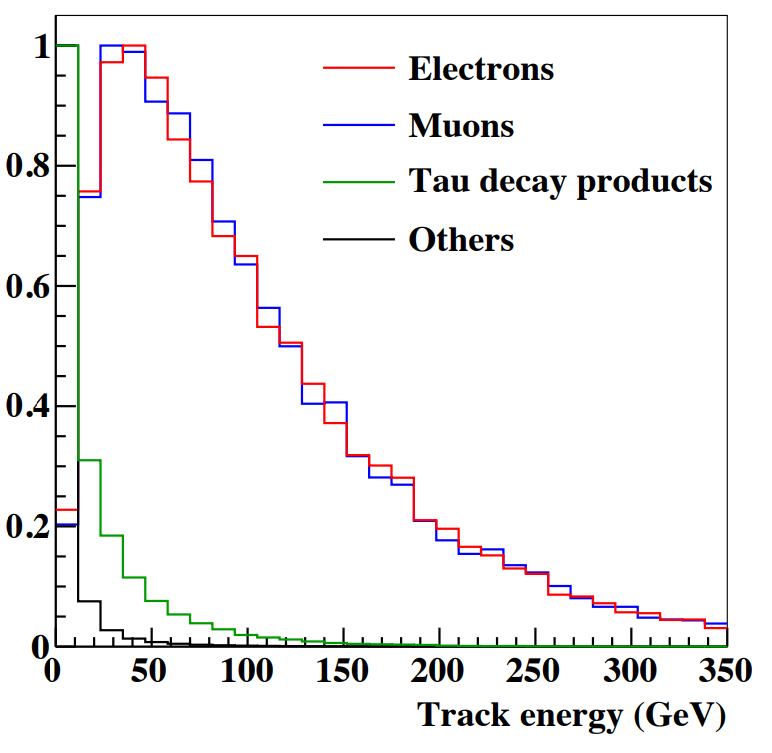
\includegraphics[width=0.55\textwidth]{../Pictures/Analysis/track-energy.png}
	\caption{Plots of the track energy for truth-matched reconstructed electrons, muons and tau decay products, and all other reconstructed particles that were not truth-matched to a lepton.}
	\label{figure:analysis/leptons/track-energy}
\end{figure}

Leptons produced within jets will be detected within the same region as the other particles from the same jet, in a high-occupancy region of the detector. Therefore, an isolated lepton detected away from the core of an identified jet is more likely to have originated from the decay of a W boson, rather than from a jet.

The impact parameter (\acrshort{IP-analysis}) is the distance between the primary vertex that produced a particle, and the closest approach of the particle's track. Electrons and muons produced from W boson decays have much lower \acrshort{IP-analysis}s than other particles or tau decay products. The impact parameter can be considered in either the longitudinal ($Z_0$) or radial ($d_0$) \footnote{This is in a cylindrical co-ordinate system, with the central axis of the cylinder along the interaction point of the detector.} components, which can be combined for a 3D \acrshort{IP-analysis}:

\begin{equation}
	\centering
	R_0 = \sqrt{Z_0^2 + d_0^2}
\label{eq:impact-parameter}
\end{equation}
% Add somewhere that all samples used include overlay of beam-related backgrounds. (If I remember correctly - and please check - it's often equivalent to 60 bunch crossings)

Figure \ref{figure:analysis/leptons/impact-parameter} shows the distribution of the three impact parameter variables for truth-matched electrons and muons.

\begin{figure}[p]
	\centering
	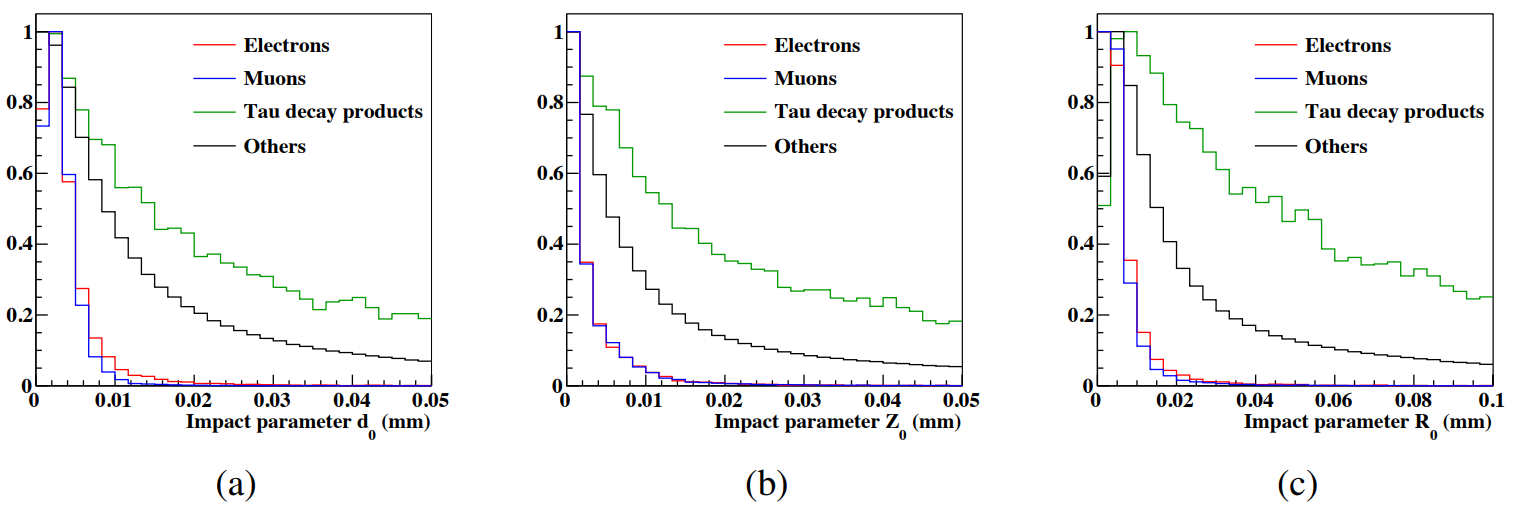
\includegraphics[width=1.0\textwidth]{../Pictures/Analysis/impact-parameter.png}
	\caption{Plots of the impact parameters $d_0$, $Z_0$, and $R_0$ for truth-matched reconstructed electrons, muons and tau decay products, and all other reconstructed particles that were not truth-matched to a lepton.}
	\label{figure:analysis/leptons/impact-parameter}
\end{figure}

Another property useful for distinguishing electrons and muons decaying from W bosons is the profile of their energy deposition in the calorimeters. We can define a ratio of the energy deposited in the electromagnetic calorimeter to the total energy deposited in the calorimeters:

\begin{equation}
	R_{CAL} = \frac{E_{CAL}}{E_{ECAL} + E_{HCAL}}
\label{eq:calorimeter-ratio}
\end{equation}

Since electrons are contained within the \acrshort{ECAL}, their value of $R_{CAL}$ will peak at 1. Muons deposit their energy throughout both calorimeters, so will peak at approximately 0.2 (see Fig. \ref{figure:analysis/leptons/cal-energy}). Taus cannot be identified this way, as their decay products do not deposit predictable amounts of energy in the calorimeters. Fig. \ref{figure:analysis/leptons/cal-energy} shows the separation of electrons and muons from other particles using $R_{CAL}$.

% Specify that these have unit normalisation.
\begin{figure}[p]
	\centering
	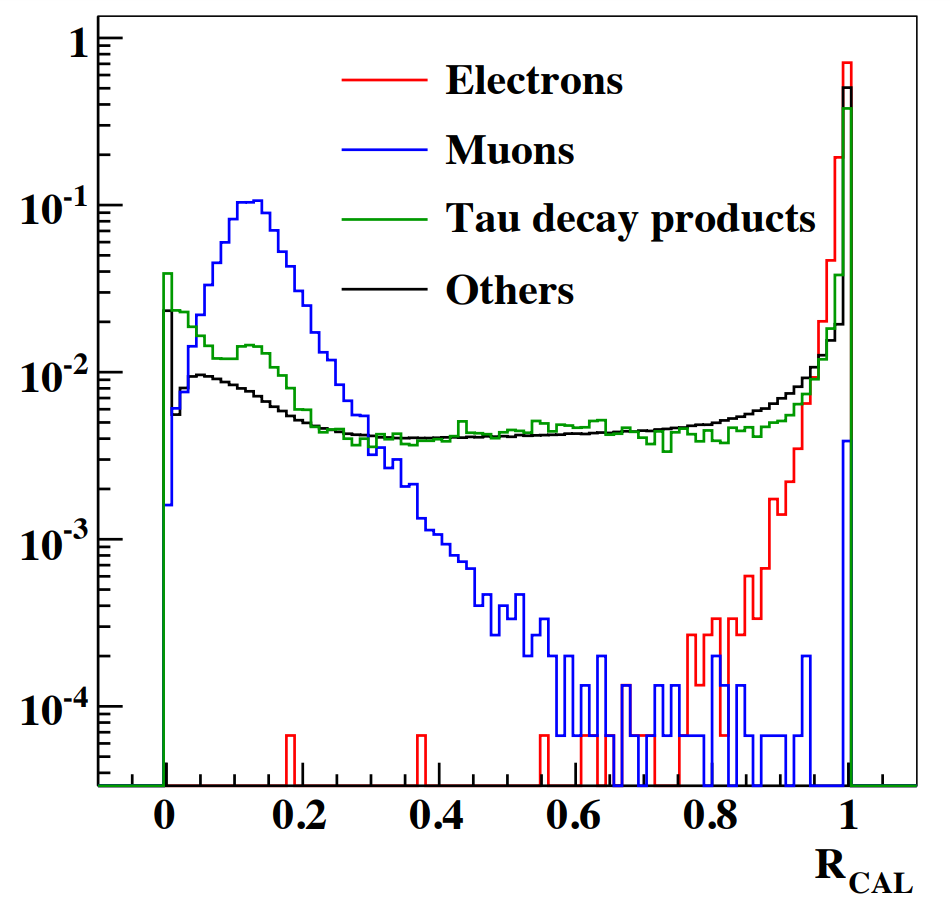
\includegraphics[width=0.55\textwidth]{../Pictures/Analysis/cal-energy.png}
	\caption{Plot of the calorimeter energy ratio $R_{CAL}$ for truth-matched reconstructed electrons, muons and tau decay products, and all other reconstructed particles that were not truth-matched to a lepton. Electrons and muons from W boson decays can be clearly distinguished from each other, and from  other particles.}
	\label{figure:analysis/leptons/cal-energy}
\end{figure}

\subsubsection{IsolatedLeptonFinder}
To perform the selections to find isolated leptons, the \texttt{IsolatedLeptonFinder} processor within \textsc{Marlin} was used. This lepton finder processor uses criteria based on the properties described above to identify isolated leptons:

\begin{itemize}
	\item Track energy greater than 15 GeV (Fig. \ref{figure:analysis/leptons/track-energy})
	\item Each of $d_0$, $Z_0$ and $R_0$ less than 0.05 mm (Fig. \ref{figure:analysis/leptons/impact-parameter})
	\item $R_{CAL}$ greater than 0.5, or in the range 0.05-0.3 (Fig. \ref{figure:analysis/leptons/cal-energy})
\end{itemize}

With these criteria, the isolated lepton finder retains 87.3\% of reconstructed isolated electrons and muons, while accepting only 0.4\% other particles.

\subsection{Tau identification}
Taus cannot be identified directly due their extremely short lifetime ($2.9 \times 10^{-13}$s), and must instead be identified from their decay products, which can vary significantly. Taus most commonly decay hadronically into an odd number number of charged or neutral pions, or leptonically into a lepton-neutrino pair; in each case always also producing at least one undetectable tau neutrino. 

Identification of taus was done using the \texttt{TauFinder} processor\cite{taufinder} within \textsc{Marlin}, which was adapted for this analysis. The criteria were determined using truth-matching the simulation data to find the best strategy to identify taus.

The processor looks at particles that may have decayed from taus, and forms a tau candidate based on their properties. First it creates a seed track with a $p_T$ greater than 10 GeV, adding all particles within a 0.04 rad cone of the seed track to the tau candidate if every particle has $p_T >$ 2 GeV and $R_0$ within the range 0.01-0.05mm. The reconstructed tau candidate must then be formed of an odd number of charged tracks, with an invariant mass of less than 1.5 GeV. This mass is slightly lower than the true tau invariant mass to account for missing energy in the form of the tau neutrinos. Then an isolation ring is defined in the region 0.04-0.24 rad around the tau candidate seed track. In order to be considered a tau, there must be fewer than five particles in the isolation ring, with a total energy of less than 5 GeV.
% If possible and straightforward, add plot to support these criteria, or give reference to where they were devised.

\subsection{Jet clustering}
Any detected isolated leptons are removed from the event, then the event is run through jet clustering using the $k_t$ algorithm \cite{kt-jet-clustering} with $R = 1.0$. The algorithm is run in exclusive mode, forcing the event into a specific number of jets -- in  the case of the hadronic analysis, eight jets -- plus an additional two beam jets, which are determined by finding the two jets with the lowest angles relative to the beam axis. The beam jets are due to beam-beam backgrounds, and once they have been identified they are removed. Once this is complete, the jet particles are then reclustered using the Durham algorithm \cite{durham-jet-clustering}.

\subsection{Flavour tagging}
\label{section:flavour-tagging}
The majority of the backgrounds for this analysis do not have four b-jets in the final state. Therefore reliable b-tagging is an important source of discriminating power.

For this analysis, b-tagging is done in the LCFIPlus package \cite{lcfiplus}, tuned using simulated samples of $e^+ e^- \rightarrow qqqqqq$ where all quarks have the same flavour. The high number of jets in the final state means that the kinematic properties of the jets are similar to those in the analysis samples. Four \acrfull{BDT} are trained for b-tagging, and four for c-tagging, trained using jet properties. These \acrshort{BDT}s then give b-tag and c-tag probabilities for each jet, which are used for event selection in the next step. % Clarify, this is what LCFIPlus itself does (not your study)?

One of the major differences in this analysis was the upgrade of the flavour-tagging, which removed a bug that influenced the performance of b-tagging \cite{clic-yukawa-coupling-2014}.

An important variable to select the signal events is the b-tag probabilities of the jets with the four highest b-tags, as well the corresponding c-tag probabilities of these four jets.

\subsection{Reconstruction of Higgs, top and W boson candidates}
\label{section:chi-squared}
After the flavour tagging is completed, the jet energies are used to reconstruct candidates for the Higgs boson, top quarks, and W bosons. The invariant masses of the tops, W bosons, and Higgs are computed, resulting in a $\chi^2$ value. By computing this $\chi^2$ value for all possible combinations of jets and finding the combination that results in the minimum, the jets can be matched to which particles produced them. The $\chi^2$ is calculated as:

\begin{equation}
  \centering
	\chi^2 = \frac{(m_{12} - m_W)^2}{\sigma^2_W} + \frac{(m_{123} - m_t)^2}{\sigma^2_{t}} + \frac{(m_{45} - m_W)^2}{\sigma^2_W} + \frac{(m_{456} - m_t)^2}{\sigma^2_{t}} + \frac{(m_{78} - m_H)^2}{\sigma^2_H}
\label{eq:chi-square}
\end{equation}
% Clarify how the resolutions in the denominators are determined; if not by you, give reference to where they come from.

where the numbered subscripts are labels for the jets used in any particular grouping. A similar equation is used for the semi-leptonic channel, using only the 6 jets present in that process. The $\chi^2$ values are extremely useful for selection, as events that are not tth, or are tth events without the fully hadronic decay channel, will have poor $\chi^2$ values, as the jets the event was forced into do not represent physical jets.

\section{Event selection}
The final event selection is done using \acrlong{BDT}, implemented in the \acrfull{TMVA} \cite{tmva}. In this method, a large number of event variables are fed into the toolkit, which are used to train \acrshort{BDT}s to distinguish signal events from background events. The generated events are split randomly into two halves. The first half is used for training the \acrshort{BDT}s, and the other becomes the samples used by the \acrshort{BDT}. In this analysis, the \acrshort{BDT}s are trained separately for each channel. % Please define training and background samples per channel

The \acrshort{BDT}s then produce a \acrshort{BDT} response value (Fig. \ref{figure:analysis/results/bdt-response}) and a value for this is chosen to optimise the event selection. The criteria for an optimal event selection is the maximal significance:

\begin{equation}
	\frac{S}{\sqrt{S + B}}
\label{eq:significance}
\end{equation}

where $S$ is the number of signal events selected, and $B$ is the number of background events selected.

For the hadronic channel, the following variables were used request, where some of these are introduced in Sections \ref{section:pfos}, \ref{section:event-shape}, and \ref{section:durham-distance}:

\begin{itemize}
	\item Reconstructed Higgs mass (Fig. \ref{figure:analysis/results/tmva-inputs-1})
	\item Number of reconstructed PandoraPFOs in the event (see \ref{section:pfos} and Fig. \ref{figure:analysis/results/tmva-inputs-1})
	\item Visible jet energy (Fig. \ref{figure:analysis/results/tmva-inputs-1})
	\item Missing transverse momentum $p_T$  (Fig. \ref{figure:analysis/results/tmva-inputs-1})
	\item $\chi^2$ of the jet grouping (see \ref{section:chi-squared} and Fig. \ref{figure:analysis/results/tmva-inputs-1})
	\item Event shape variables -- thrust, sphericity, aplanarity, and oblateness (see \ref{section:event-shape} and Figs. \ref{figure:analysis/results/tmva-inputs-1} and \ref{figure:analysis/results/tmva-inputs-2})
	\item Four highest b-tag values and their corresponding c-tags (see \ref{section:flavour-tagging} and Figs. \ref{figure:analysis/results/tmva-inputs-2} and \ref{figure:analysis/results/tmva-inputs-3})
	\item The cosine of the decay angle of the $h \rightarrow b\overline{b}$, and the cosine of the angles between the Higgs and each top quark (Fig. \ref{figure:analysis/results/tmva-inputs-3})
	\item The distance between the two closest jets, as defined by the Durham jet clustering algorithm (see \ref{section:durham-distance} and Fig. \ref{figure:analysis/results/tmva-inputs-4})
	\item The energy of the four lowest-energy jets (Figs. \ref{figure:analysis/results/tmva-inputs-4} and \ref{figure:analysis/results/tmva-inputs-5})
	\item The cosine of the angle of the two jets closest to the beam-axis 
\end{itemize}

\begin{figure}[h]
	\centering
	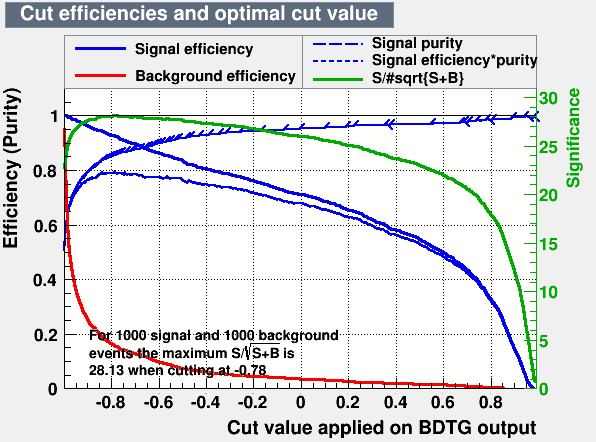
\includegraphics[width=0.75\textwidth]{../Pictures/Analysis/BDTs/mvaeffs_BDTG.png}
	\caption{Signal and background efficiencies for different values of the cut valued applied on the results of the BDTs. The green line is the plot of the significance against the cut value.}
	\label{figure:analysis/results/tmva-efficiency}
\end{figure}

\subsection{PandoraPFOs}
\label{section:pfos}
The number of particles reconstructed as Pandora\acrshort{PFO}s is highly correlated with the number of jets in the event. As the number of jets in the event is not directly measured, since the jet clustering and re-clustering forces the event into a specific number of jets, the number of \acrshort{PFO}s can be used to help infer whether the event was a signal event with 8 jets, or a background event with fewer jets.

\subsection{Event shape}
\label{section:event-shape}
% Discuss - not really - a low momentum event can have high thrust. Clarify, this is not correct. what is index i, per PFO or per jet, it makes a big difference here, need to specify. Define n as thrust major axis.
The thrust of event is an expression of the net momentum of the event. An event's thrust is given by:

\begin{equation}
	T = max \frac{\sum_i | \hat{n} \cdot \overrightarrow{p_i} |}{\sum_i | \overrightarrow{p_i} |}
\label{eq:thrust}
\end{equation}

where $p_i$ is the momentum of the jet. For example, an event with two jets emitted in exactly opposite directions would have a thrust of 1. An event with several jets that are spherically symmetric would have a thrust of 0.5. The event thrust is thus a good discriminating variable for the $t\overline{t}$ background, as this is a dijet system and will have much a larger thrust than for the signal event $t\overline{t}h$, or for similar final states like $t\overline{t}Z$ or $t\overline{t}b\overline{b}$. The effect of the event thrust can be seen in Fig. \ref{figure:analysis/results/tmva-inputs-1}.

Also used is the sphericity:

\begin{equation}
	S = \frac{\sum_i p_i^{\alpha} p_i^{\beta}}{\sum_i | p_i |^2}
\label{eq:sphericity}
\end{equation}

and the aplanarity:

\begin{equation}
	A = \frac{3}{2}\lambda_3
\label{eq:aplanarity}
\end{equation}

The effects of sphericity and aplanarity can be seen in Fig. \ref{figure:analysis/results/tmva-inputs-2}.

\subsection{Durham jet distance parameter}
\label{section:durham-distance}
The Durham jet clustering algorithm defines a distance parameter $Y_{ij}$ such that:

\begin{equation}
	Y_{ij} = \frac{min(E_i^2 , E_j^2)(1-cos\theta_{ij})}{E^2_{CM}}
\label{eq:durham-distance}
\end{equation}

where $i$ represents the $n$\textsuperscript{th} jet, and $j$ represents the $(n+1)$\textsuperscript{th} jet. When the event is forced into an incorrect number of jets -- such as when a $t\overline{t}$ event is clustered into eight jets as if it were a fully hadronic $t\overline{t}h$ event -- the values of the distances $Y_{45}$, $Y_{56}$, and $Y_{67}$ will be smaller than in true eight-jet final states. \\

\begin{figure}[p]
	\centering
	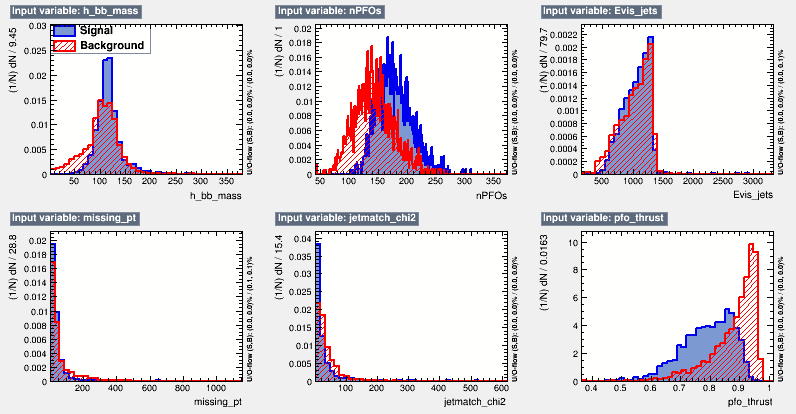
\includegraphics[width=1.0\textwidth]{../Pictures/Analysis/BDTs/variables_id_c1.png}
	\caption{Input variables for the BDTs: Higgs mass from $b\overline{b}$ jets; number of particle flow objects; visible jet energy; missing transverse momentum; $\chi^2$ value from jets (from Eq. \ref{eq:chi-square}); event thrust.}
	\label{figure:analysis/results/tmva-inputs-1}
\end{figure}

\begin{figure}[p]
	\centering
	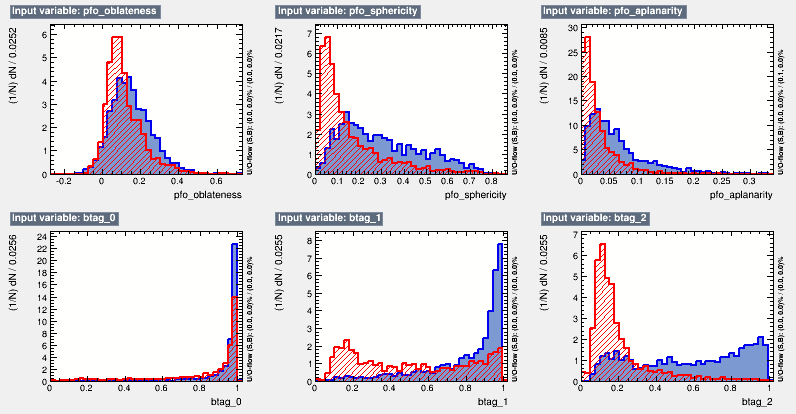
\includegraphics[width=1.0\textwidth]{../Pictures/Analysis/BDTs/variables_id_c2.png}
	\caption{Input variables for the BDTs: event oblateness; event sphericity; event aplanarity; first, second and third highest b-tags.}
	\label{figure:analysis/results/tmva-inputs-2}
\end{figure}

\begin{figure}[p]
	\centering
	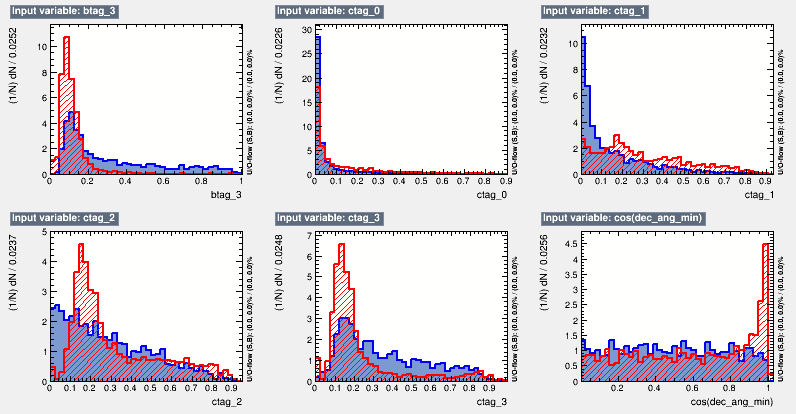
\includegraphics[width=1.0\textwidth]{../Pictures/Analysis/BDTs/variables_id_c3.png}
	\caption{Input variables for the BDTs: the fourth highest b-tag; the corresponding c-tags of the jets with the four highest b-tags; the cosine of the Higgs decay angle.}
	\label{figure:analysis/results/tmva-inputs-3}
\end{figure}

\begin{figure}[p]
	\centering
	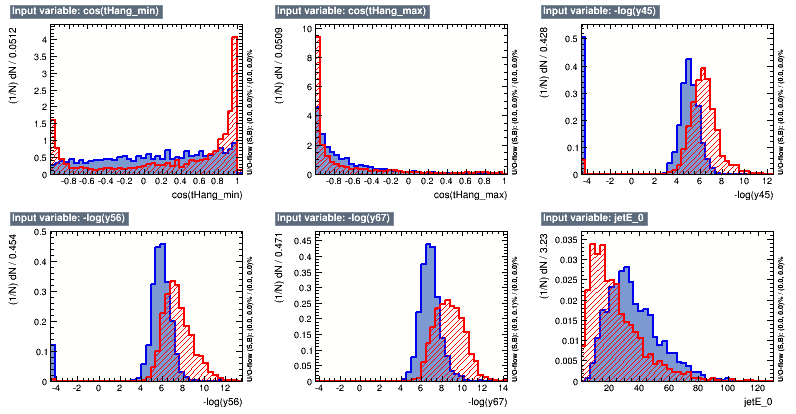
\includegraphics[width=1.0\textwidth]{../Pictures/Analysis/BDTs/variables_id_c4.png}
	\caption{Input variables for the BDTs: the cosine of the minimum and maximum angles between the top quark and Higgs boson; the Durham distance values $Y_{45}$, $Y_{56}$, and $Y_{67}$; lowest jet energy}
	\label{figure:analysis/results/tmva-inputs-4}
\end{figure}

\begin{figure}[h]
	\centering
	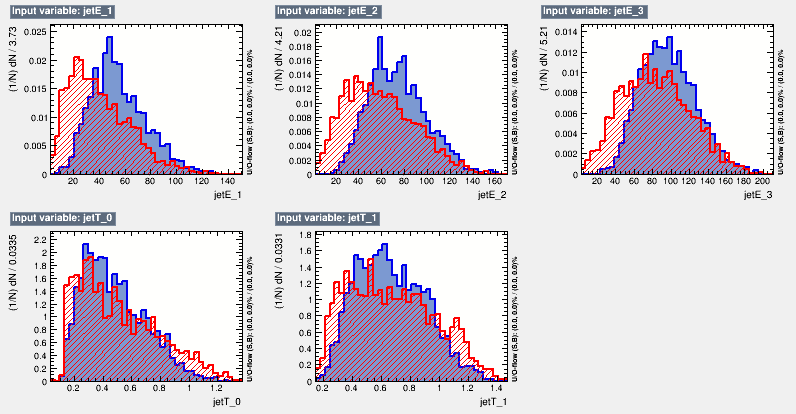
\includegraphics[width=1.0\textwidth]{../Pictures/Analysis/BDTs/variables_id_c5.png}
	\caption{Input variables for the BDTs: second, third, and fourth lowest jet energies; the transverse momentum of the first and second jets.}
	\label{figure:analysis/results/tmva-inputs-5}
\end{figure}

\begin{table}[ht]
\centering
	\begin{tabular}{ l r r r }
	\hline \hline
	\textbf{Process} & \textbf{$N$} & \textbf{Fully hadronic} & \textbf{Semi-leptonic} \\ \hline
	$t\overline{t}h$, 6 jets, $h \rightarrow b\overline{b}$ & 647 & 367 & 38 \\
	$t\overline{t}h$, 4 jets, $h \rightarrow b\overline{b}$ & 623 & 1 & 270 \\ \hline
	$t\overline{t}h$, 2 jets, $h \rightarrow b\overline{b}$ & 150 & 2 & 22 \\

	$t\overline{t}h$, 6 jets, $h \not\rightarrow b\overline{b}$ & 473 & 54 & 11	 \\
	$t\overline{t}h$, 4 jets, $h \not\rightarrow b\overline{b}$ & 455 & 8 & 22\\
	$t\overline{t}h$, 2 jets, $h \not\rightarrow b\overline{b}$ & 110 & 0 & 1 \\

	$t\overline{t}Z$, 6 jets & 2843 & 345 & 34 \\
	$t\overline{t}Z$, 4 jets & 2738 & 59 & 217 \\
	$t\overline{t}Z$, 2 jets & 659 & 1 & 16 \\
	
	$t\overline{t}b\overline{b}$, 6 jets & 824 & 326 & 26 \\
	$t\overline{t}b\overline{b}$, 4 jets & 794 & 57 & 226 \\
	$t\overline{t}b\overline{b}$, 2 jets & 191 & 2 & 18 \\

	$t\overline{t}$ & 203700 & 498 & 742 \\ \hline

	total $t\overline{t}H$ signal & 2458 & 433 (17.6\%) & 365 (14.8\%) \\ 
	total background & 211749 & 1287 (0.61\%) & 1280 (0.60\%) \\
	Significance &   & 10.44 & 9.00 \\ \hline \hline

	\end{tabular}
	\caption{Expected numbers of signal and background events classified by the \acrshort{BDT}s as either fully hadronic or semi-leptonic in 1.5 ab\textsuperscript{-1} at $\sqrt{s}$ = 1.4 TeV.}
	\label{table:physics/SM/selections}
\end{table}

\section{Results}
In order to find the value of the cut on the \acrshort{BDT} response  that gives the maximal significance, the different possible values are looped over. A plot of the MVA cut against the sigificance can be found in Fig. \ref{figure:analysis/results/tmva-efficiency}. For the the fully hadronic channel, the cut giving the maximum significance was found to be $>$ 0.181. This corresponds to a significance of 10.44. The result of of applying this selection to the BDT response on the event samples can be seen in Table \ref{table:physics/SM/selections}.

The sensitivity to the top-Higgs Yukawa coupling can then be calculated directly by taking the inverse of the signal significance. With a signal significance of 10.44 in the hadronic channel, the precision on the cross-section is found to be 9.6\%. A similar analysis for the semi-leptonic channel found a signal significance of 9.0 and thus a precision on the cross-section of 11.1\%. The combined uncertainty for the cross-section of both decay channels is: $\Delta\sigma$ = 7.5\%.

In order to use the precision on the measurement of the cross-section to calculate the precision on the measurement of the top-Higgs Yukawa coupling, the contribution of the higgstrahlung diagram must be taken into account, as explained in Section \ref{section:higgstrahlung}. The value of $\kappa$ had been determined to be 0.503, therefore the uncertainty on the top-Higgs Yukawa coupling is:

\begin{equation}
	\frac{\Delta y_t}{y_t} = 0.503 \frac{\Delta\sigma}{\sigma} = 3.8\%
\label{eq:result-coupling}
\end{equation}

This represents an improvement over the previous study \cite{clic-yukawa-coupling-2014} where the cross-section could be measured with an accuracy of 10.8\% in the fully hadronic channel and 12.0\% in the semi-leptonic channel, giving a combined precision of 8.1\%. This then translated to the precision on the coupling of 4.27\%. Therefore the study presented above represents an improvement of almost 11\% from the previous analysis.

These studies also represent a significant increase over the precision the \acrshort{LHC} experiments. The full \acrshort{LHC} programme, including the high luminosity upgrade (\acrshort{HL-LHC}), is expected to accumulate 3000 fb\textsuperscript{-1} of data at $\sqrt{s}$ = 14 TeV, and achieve an uncertainty on the top-Higgs Yukawa coupling of between 7-10\% \cite{lhc-top-yukawa}.

% Give reference for "under 10%", e.g. from [43]
The systematic uncertainties for this study from flavour tagging, lepton reconstruction, and jet energy scale are all expected to be below 10\%, making them significantly smaller than the statistical uncertainty of the cross-section.  \\

%\begin{figure}[h]%
%	\centering
%    \subfloat{{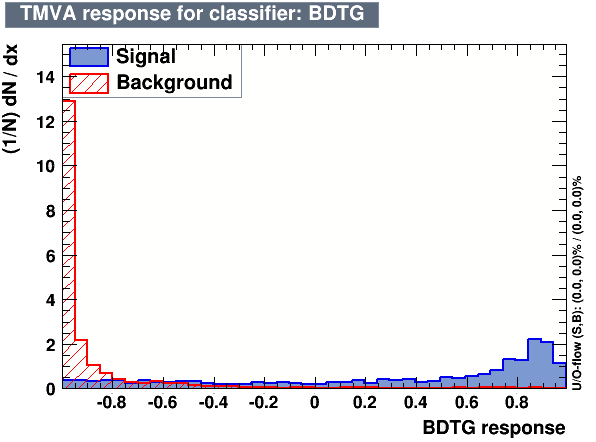
\includegraphics[width=0.45\textwidth]{../Pictures/Analysis/BDTs/mva_BDTG.png} }}%
%    \qquad
%	\subfloat{{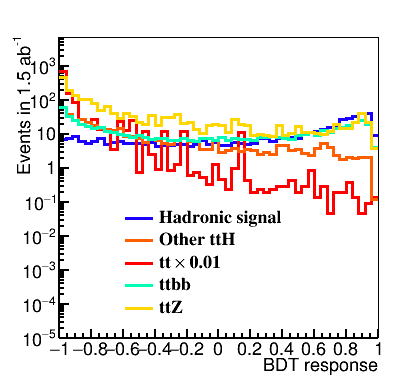
\includegraphics[width=0.45\textwidth]{../Pictures/Analysis/BDTs/MVA_BDTG_comb_had.png} }}%
%    \caption{Normalised BDTG response for signal and background (left); and BDTG scaled to the number of events expected in 1.5 ab\textsuperscript{-1} (right).}%
%    \label{figure:analysis/results/bdt-response}%
%\end{figure}

\begin{figure}[h]
	\centering
	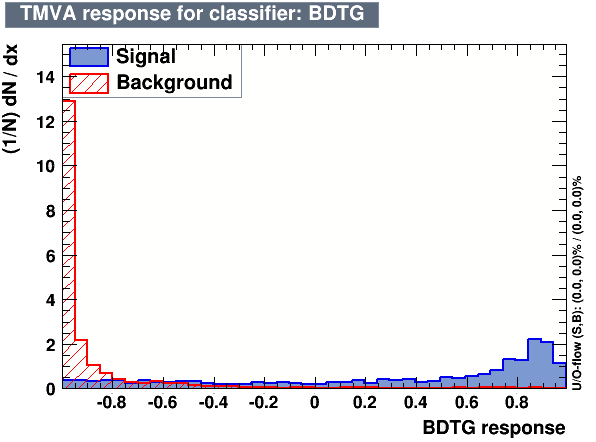
\includegraphics[width=0.65\textwidth]{../Pictures/Analysis/BDTs/mva_BDTG.png}
	\caption{Normalised BDTG response for signal and background.}
	\label{figure:analysis/results/bdt-response}
\end{figure}

% Comment on the structure of the tt distribution. As discussed in viva, I expect this is do to tt being a large, high cross-section process and so the number of events simulated corresponds to a lower lumi than that of other sources, and therefore every event that get through the selection carries a higher weight.  If unclear, please ask us.
\begin{figure}[h]
	\centering
	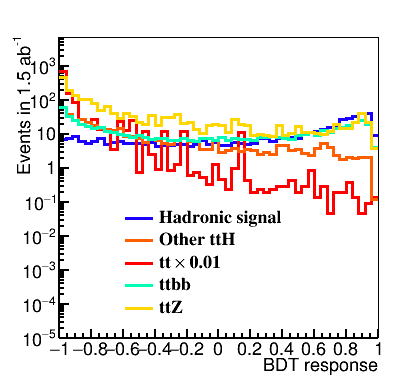
\includegraphics[width=0.60\textwidth]{../Pictures/Analysis/BDTs/MVA_BDTG_comb_had.png}
	\caption{BDTG scaled to the number of events expected in 1.5 ab\textsuperscript{-1}.}
	\label{figure:analysis/results/bdt-response}
\end{figure}